\pagebreak
\subsection{Ground Support Equipment}\label{sec:4.9}
The purpose of the ground station was to monitor in real-time the experiment and provide manual override capability in case the experiment failed functioning autonomously. The manual override was able to control all the valves, pump, and heaters. It also provided a service to change the sampling schedule while in flight. \par
One personal computer was used to connect to the E-Link through the Ethernet port. A GUI was created to display the sensors data and valves, pump states during the experiment. MATLAB GUIDE was used for the development. \par
The design of the ground station was responsible for receiving and transmitting data over the provided Ethernet connection. Using GUIDE to create a GUI and respective functions as a skeleton, the necessary  functionality to receive, transmit and display were built accordingly. The functions were defined for each GUI element.
\begin{figure}[H]
    \centering
    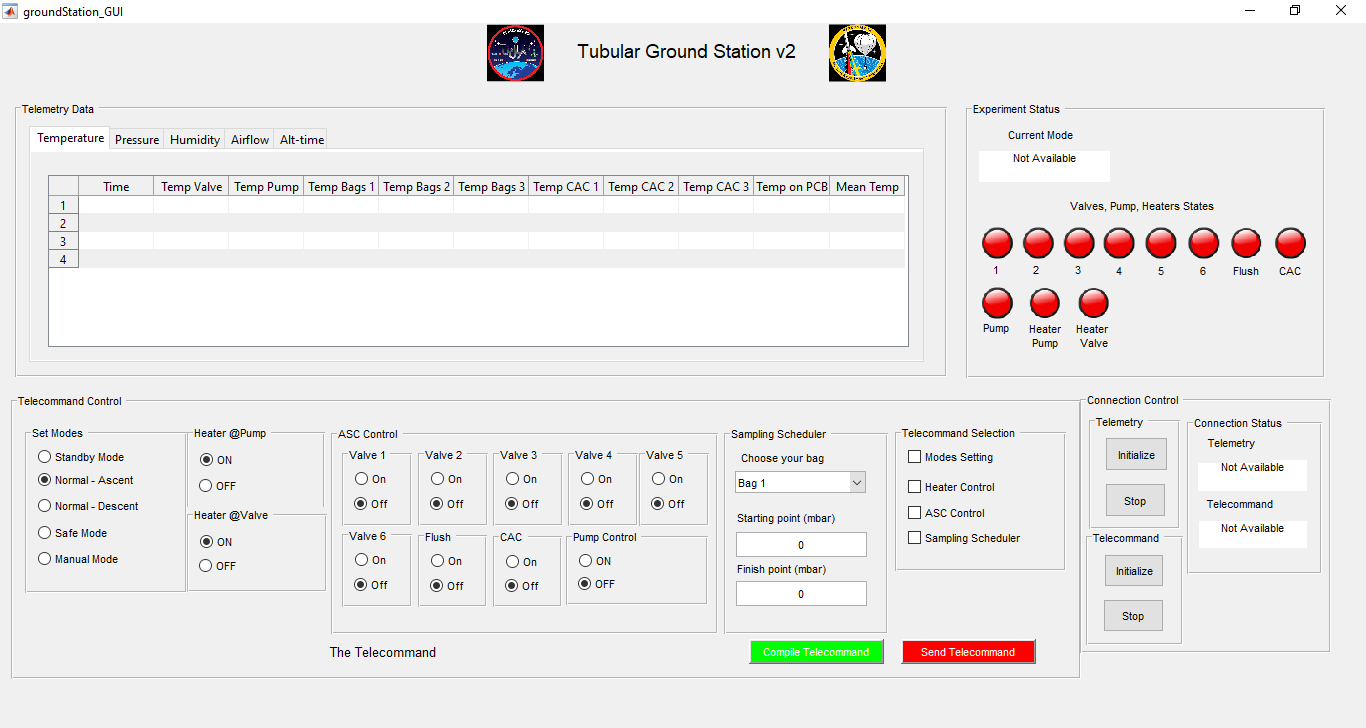
\includegraphics[width=0.8\textwidth]{4-experiment-design/img/GS-GUI-final.png}
    \caption{GUI Design for Ground Station Version 2.}
    \label{fig:guiDesign}
\end{figure}
Figure \ref{fig:guiDesign} shows the design of ground station GUI. Telemetry data was shown in several tables based on the data type. The data was recorded and stored on the computer. The experiment status panel represented the real-time status of the experiments, the red indicator changed to green if the pump or valves were open later on. On the bottom side, the telecommand control panel provided command generation for the experiment. On its right side, the connection control panel had full control of the connections.


\raggedbottom